\documentclass[12pt, a4paper]{article}

\usepackage{array}
\usepackage[portuguese]{babel}
\usepackage{chngpage}
\usepackage{float}
\usepackage[a4paper, margin=2cm]{geometry}
\usepackage{graphicx}
\usepackage{hyperref}
\usepackage{setspace}
\usepackage{xcolor}

\title{\Huge \textbf{Computação Gráfica \\ \Large Trabalho Prático -- Fase I}}
\date{2 de março 2025}
\author{Grupo \textbf{\color{red} TODO}}

\begin{document}

\begin{center}
    
\includegraphics[width=0.25\textwidth]{res/cover/EE-C.eps}
\end{center}

\chardef\_=`_
\onehalfspacing
\setlength{\parskip}{\baselineskip}
\setlength{\parindent}{0pt}
\def\arraystretch{1.5}

{\let\newpage\relax\maketitle}
\maketitle
\thispagestyle{empty}

\vspace*{\fill}

\begin{adjustwidth}{-2cm}{-2cm} % These values only need to be large enough to center the table
    \begin{center}
        \begin{tabular}{>{\centering}p{0.25\textwidth}
                        >{\centering}p{0.25\textwidth}
                        >{\centering}p{0.25\textwidth}
                        >{\centering\arraybackslash}p{0.25\textwidth}}
            
\includegraphics[width=3.5cm]{res/cover/A104437.png} &
            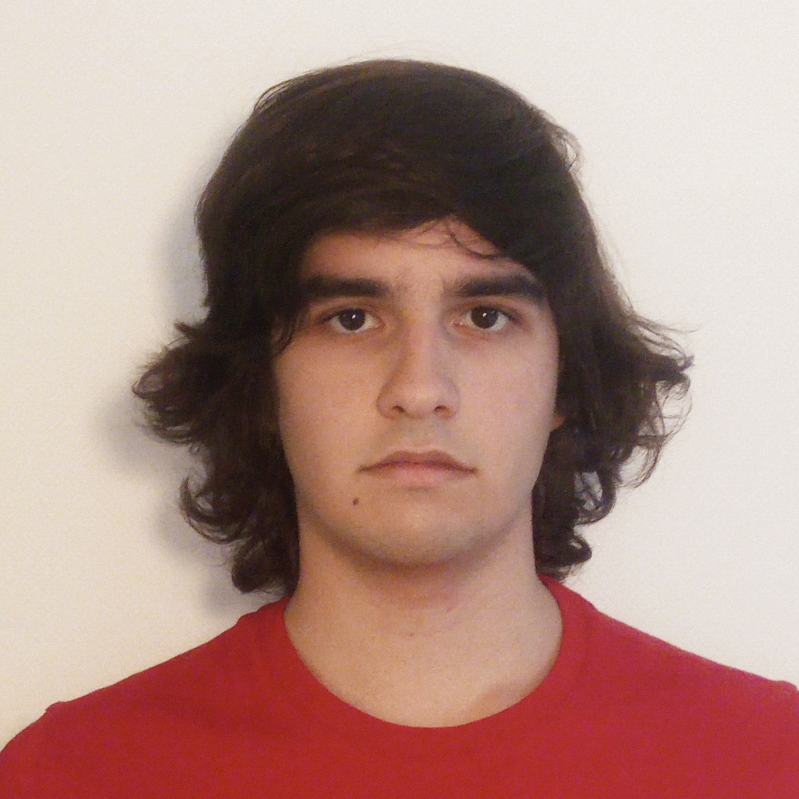
\includegraphics[width=3.5cm]{res/cover/A104348.png} &
            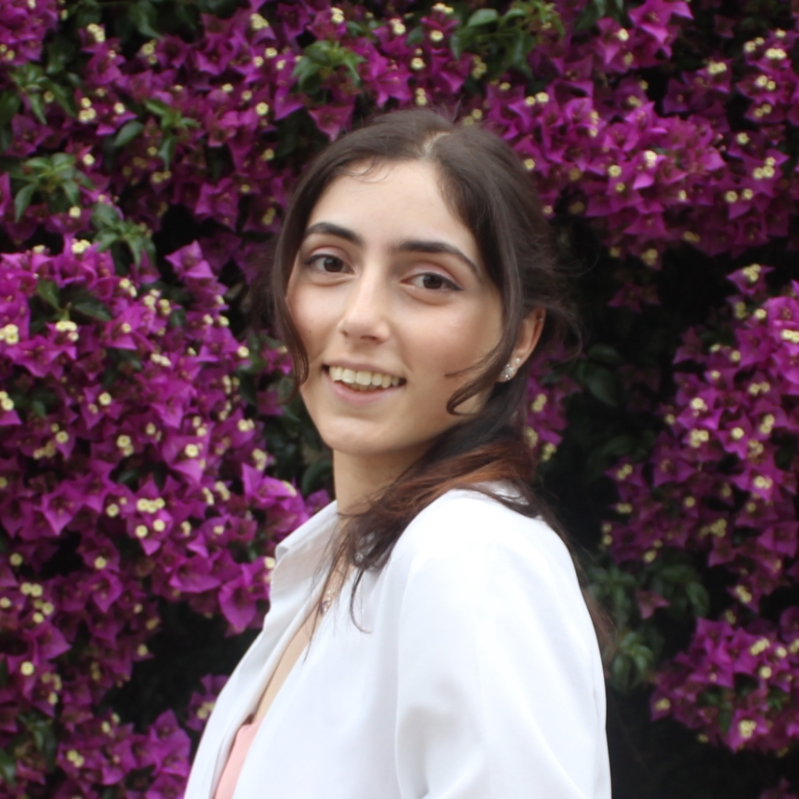
\includegraphics[width=3.5cm]{res/cover/A90817.png} &
            
\includegraphics[width=3.5cm]{res/cover/A104179.png} \\

            Ana Oliveira & Humberto Gomes & Mariana Cristino & Sara Lopes \\
            A104437      & A104348        & A90817           & A104179
        \end{tabular}
    \end{center}
\end{adjustwidth}

\pagebreak

\begin{abstract}
    \textbf{\color{red} TODO - resumo}
\end{abstract}

\section{\emph{Generator}}

\textbf{\color{red} TODO - \emph{generator}}

\section{\emph{Engine}}

\subsection{Cena (Scene)}

A classe \texttt{Scene} assume um papel importante, pois interpreta e organiza as informações
contidas no ficheiro de cena \texttt{XML}. A biblioteca \texttt{TinyXML2} é a ferramenta utilizada
para analisar a estrutura do ficheiro, permitindo à \texttt{Scene} extrair dados importantes como as
dimensões da janela de visualização, as propriedades da câmara e a lista de entidades a serem
renderizadas.

O ficheiro de cena \texttt{XML} serve como um guião para a engine, define a estrutura e o conteúdo
da cena a ser renderizada. A sua estrutura hierárquica permite a organização de objetos em grupos,
facilitando a criação de cenas complexas.
O processo de análise inicia-se com a leitura do elemento raiz \texttt{<world>}, que contêm todos os
elementos de configuração. A \texttt{Scene} extrai as dimensões da janela a partir do
elemento \texttt{<window>}, definindo a largura e altura da área de renderização. As propriedades da
câmara, incluindo a sua posição no espaço, o ponto para o qual está a olhar (\texttt{lookAt}), o
vetor que define a sua orientação vertical (\texttt{up}), o campo de visão (\texttt{FOV}) e os
planos de recorte próximo e distante, são obtidas do elemento \texttt{<camera>}.

Os elementos \texttt{<group>} podem conter outros elementos \texttt{<group>} ou elementos
\texttt{<models>}, que especificam os modelos 3D a serem carregados e renderizados. Esta organização
hierárquica facilita a criação de cenas complexas, onde objetos podem ser agrupados e transformados
em conjunto.

O carregamento dos modelos 3D é realizado de forma eficiente, com recurso a um
\texttt{std::unordered\_map} para armazenar os modelos já carregados. Quando um elemento
\texttt{<model>} é encontrado, o ficheiro especificado no atributo \texttt{file} é lido.
Se o modelo já foi carregado anteriormente, ele é reutilizado; caso contrário, um novo modelo é
carregado e armazenado no mapa. Esta estratégia evita a duplicação de dados e melhora o desempenho
da engine.

Cada modelo é encapsulado numa instância da classe \texttt{Entity}, que representa um
objeto na cena. A \texttt{Scene} mantém uma lista de \texttt{std::unique\_ptr<Entity>}, assegurando
a gestão eficiente da memória das entidades. A utilização de \texttt{std::unique\_ptr} assegura que
as entidades são destruídas automaticamente quando a cena é destruída.

A cena interage com outros componentes da engine para renderizá-la corretamente. A câmara,
representada pela classe \texttt{Camera}, fornece a matriz de visualização e projeção, que é
utilizada pela \texttt{RenderPipeline} para transformar os vértices dos modelos.

A organização modular da engine permite a fácil expansão e manutenção do código, facilitando a
adição de novas funcionalidades e a otimização do desempenho.

\subsection{Entidade (Entity)}

A classe \texttt{Entity} representa um objeto 3D individual na cena, combina um modelo
(\texttt{Model}) com uma cor associada. Esta é responsável por renderizar o modelo com recurso à
\textit{pipeline} de renderização (\texttt{RenderPipeline}).

O construtor da \texttt{Entity} recebe um \texttt{std::shared\_ptr<Model>} e um \texttt{glm::vec4}
representando a cor da entidade. O modelo é armazenado internamente, e a cor é utilizada durante a
renderização. A utilização de um \texttt{std::shared\_ptr} permite que múltiplos objetos na cena
partilhem o mesmo modelo, reduzindo o consumo de memória.

O método \texttt{draw} da entidade recebe uma referência à \texttt{RenderPipeline} e realiza a
renderização do modelo. Primeiro, a cor da entidade é definida na \textit{pipeline}, com recurso ao
método \texttt{setColor}. Em seguida, o método \texttt{draw} do \texttt{Model} é chamado para
renderizar o modelo no ecrã.

A separação entre \texttt{Scene} e \texttt{Entity} promove uma organização clara e modular do código
, facilitando a criação e gestão de cenas complexas. A \texttt{Scene} lida com a interpretação do
ficheiro \texttt{XML} e a organização das entidades, enquanto a \texttt{Entity} é responsável pela
renderização individual de cada objeto.

\section{Resultados obtidos}

\textbf{\color{red} TODO - resultados}

\section{Conclusão e Trabalho Futuro}

\textbf{\color{red} TODO - conclusão}

\begingroup
\section{Bibliografia}
\renewcommand{\section}[2]{}

\begin{thebibliography}{9}
    \bibitem{exemplo}
        \href{https://youtu.be/dQw4w9WgXcQ}{Um item de exemplo na bibliografia}
\end{thebibliography}
\endgroup

\end{document}
